La agricultura enfrenta desafíos crecientes en la optimización de la
productividad y la eficiencia, especialmente en regiones con condiciones
climáticas adversas y variables. Los sistemas de cultivo tradicionales suelen
ser ineficientes en la gestión de recursos esenciales como agua, nutrientes y
energía, en gran parte debido a la falta de monitoreo en tiempo real, lo que
afecta negativamente tanto la calidad como el rendimiento de los cultivos.
Además, los agricultores se enfrentan a altos costos operativos y a un impacto
negativo en la sostenibilidad ambiental debido a prácticas no optimizadas. Ante
estas dificultades, los cultivos en invernaderos han surgido como una solución
mejorada, permitiendo un mayor control sobre las condiciones ambientales y una
utilización más eficiente de los recursos.

Este trabajo se desarrolla en colaboración con Wentux, una empresa argentina
que, desde 2018, se dedica al desarrollo de soluciones tecnológicas basadas en
IoT (\textit{Internet of Things}) para la gestión del clima en invernaderos. La
iniciativa surge a partir del programa de vinculación con empresas del
posgrado, que busca fomentar la colaboración entre el sector académico y el
ámbito empresarial. Wentux ofrece productos que permiten controlar de manera
automatizada el clima de los cultivos mediante el uso de sensores y actuadores.

Actualmente, los sistemas de Wentux están compuestos por un nodo central con
conexión Wi-Fi y sensores y actuadores conectados de forma cableada, lo cual
limita la flexibilidad y escalabilidad de la solución. Los datos del sistema se
visualizan a través de una página web integrada en el nodo central, y el
monitoreo y control se realizan únicamente de manera local.

La propuesta, como puede observarse en la figura \ref{fig:diagBloques},
consiste en desarrollar una red Mesh (malla) de sensores y actuadores
inalámbricos basados en el ESP32-C3, que se conectan a un módulo central
mediante tecnología BLE (\textit{Bluetooth Low Energy}). Este módulo, también
basado en un ESP32-C3, se conecta a Internet vía Wi-Fi y envía los datos a un
servidor IoT a través del protocolo MQTT (\textit{Message Queue Telemetry
	Transport}). Esto permitirá monitorear y gestionar el sistema de manera remota
desde una aplicación web del tipo SPA (\textit{Single Page Application}).

\begin{figure}[htpb]
	\centering
	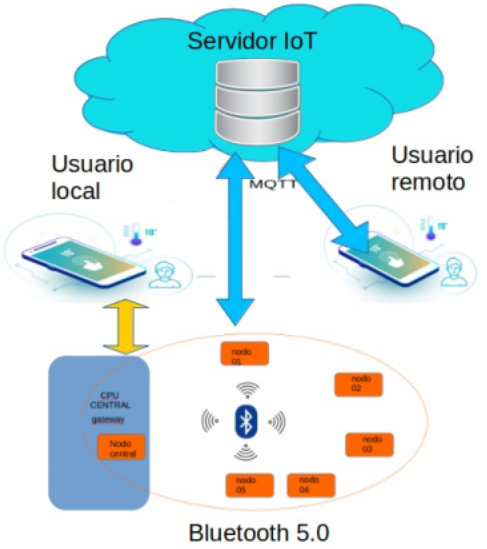
\includegraphics[width=.85\textwidth]{./Figuras/figura1.png}
	\caption{Diagrama en bloques del sistema.}
	\label{fig:diagBloques}
\end{figure}

Esta solución ofrece a los clientes finales un mayor control sobre sus
cultivos, mejora la eficiencia en la gestión del clima y optimiza los recursos,
lo que se traduce en una mayor productividad y una reducción de los costos
operativos.